\section{Set up} 

1+1 dimensional spacetime, two charges $q, -q$
are set at $x^1=0, x^{1}=a$, respectively. Ignoring vacuum polarization effects,
this yields a constant electric field of strength $q$ pointing towards positive $x^{1}$.
We study the solutions to the semiclassical Klein-Gordon-Maxwell equations
\begin{subequations}
    \begin{align}
        \left( D_\mu D^\mu + m^2 \right)\phi &= 0, \\
        \label{eq:KG}
        \partial_\mu F^{\mu\nu} &= \left< j^\nu \right>_\Omega,
        \label{eq:Maxwell}
    \end{align}
\end{subequations} in the region $x \in     \mathbb{R} \times [0,
a]$. Here, $D_\mu = \partial_\mu +ie A_\mu$ defines the gauge covariant
derivative, \begin{align}
    j^\nu = \frac{ie}{2} \left((D^\nu \phi^*) \phi - \phi^*
    D^\nu \phi \right)
\end{align}
is the charge current density of the Klein-Gordon field, and
$\left< \right>_{\Omega}$ takes its expectation value with
the scalar field in the state $\Omega.$ 
The solutions looked for are the Maxwell tensor $F^{\mu
\nu}$ and the two-point function of the vacuum state $\Omega$. Following
\cite[]{Ambjorn:1981xv, Wernersson:2020xeh}, the metric signature
is $(+,-)$.

In choosing the Coulomb gauge $\partial_1 A_1=  0$, the spatial component
of $A_\mu$ will in general be a constant that is gauged away to 0. Setting $\nu =0$ in Eq.~\eqref{eq:Maxwell} yields the Poisson equation for the electrostatic potential $A_0$
\begin{align}
    \partial_1^2 A_0(x^1) =  -\rho, \label{eq:poisson}
\end{align} 
with 
\begin{align}
    \rho =  \left< j^0 \right>_0 = \frac{ie}{2} \bra{0} (\partial_1
    \phi^*) \phi -\phi^* \partial_1 \phi \ket{0}
\end{align}
the vacuum polarization, i.e. the vacuum expectation value (VEV)\marginnote{In case the words VEV turn up again.} of the zeroth component of the charge current density. $\ket{0}$ is the vacuum state of the scalar field. 
Eq. \eqref{eq:poisson} will be solved with the boundary conditions
\begin{align}
    \left. \partial_1
        A_0(x^1)\right|_{x^1=0, a} =  -q
        \label{eq:A0-boundary-conditions}
\end{align}
so that a measurement of the electric
field close to the boundary is not screened by the vacuum polarization.
This fixes the solution to Eq.~\eqref{eq:poisson} up to an addition constant,
which is conveniently chosen so that $A_0(\frac{a}{2}) = 0$. For a given charge
density $\rho(x^{1})$, Eq.~\eqref{eq:poisson} is solved by
\begin{align}
        A_0(x^1) = -q\left(x^1 - \frac{a}{2} \right) -
        \int_{\frac{a}{2}}^{x^{1}} \int_{0}^{\chi} \rho(\xi) d \xi d \chi.
    \label{eq:A0-general} 
\end{align}


\section{Field modes}

In the chosen gauge, the Klein-Gordon equation is of the form \begin{align}
    \left[ (\partial_0 + ie A_0 )^2 + \partial_1^2 - m^2
    \right]\phi = 0,
    \label{eq:TDKGE}
\end{align}
which will be studied using different boundary conditions. We will consider Dirichlet  $\left.\phi \right|_{x^{1}=0,a} = 0$ and Neumman $\left.\partial_{1} \phi\right|_{x^1=0,a }=0$ boundary conditions, although more general Robin boundary conditions may be considered.

With the single frequency ansatz $\phi_n(x) = \phi_n (x^{1}) e^{-i\Omega_n x^0}$,
Eq.~\eqref{eq:TDKGE} is split into ordinary differential equations for each 
of the modes
\begin{align}
    \left[ (\Omega_n - e A_0 )^2 + \partial_{1}^2 -  m^2 \right]\phi_n
    = 0,
    \label{eq:TIKGE}
\end{align}
where the frequencies $\Omega_n$ are gauge dependent and to be determined by
the boundary conditions.

Following \cite{Ambjorn:1981xv}, the following dimensionless parameters
are defined 
\begin{itemize}
    \item $z = \frac{Z}{a}$,
    \item $\lambda = e E a^2,$
    \item $\varepsilon = ea$,
    \item $\omega_{n} = a\Omega_{n, \alpha} + \lambda \alpha$,
\end{itemize}
where $\alpha \in \mathbb{R}$ is a parameter characterizing
global gauge transformations of the form \begin{align}
    \varepsilon A_0 \to \varepsilon A_0 + \lambda\alpha.
\end{align} This way, the mode energies $\omega_n$ are ensured to be gauge invariant,
and Eq.~\eqref{eq:TIKGE} takes the form \begin{align}
    \left[ (\omega_n - \varepsilon A_0 )^2 + \frac{d^2}{dz^2} - a^2
    m^2\right] \phi_n = 0.  \label{eq:mode-equation}
\end{align}
The modes $\phi_n$ are normalized with respect to the symplectic
norm
\begin{align}
    (\phi_n, \phi_m) = i\int_{0}^{1} (\phi_n^* \pi_m^* - \pi_n \phi_m)dz,
\end{align}
with $\pi_n = (D_0 \phi_n)^*$ the canonical conjugate of
$\phi_n$.

The general solution to Eq.~\eqref{eq:TDKGE} is thus decomposed in
modes \begin{align}
    \phi(t, z) = \sum_{n>0}^{} a_n \phi_n(z) e^{-i\omega_n t} +
    \sum_{n<0}^{} b^\dagger_n \phi_n(z) e^{-i\omega_n t},
\end{align} where positive (negative) values of $n$ correspond to modes of positive
(negative) norm. $a_n$ and $b_n$ are the ladder operators for the positive and
negative norm solutions, respectively, obeying the commutation relations
\begin{align*}
    [a_n, a_n^\dagger ] = [b_n, b_n^\dagger ] =\delta_{nm}
\end{align*}
and all other commutators vanishing. The ladder operators define
the vacuum state $\ket{0}$ as that for which $a \ket{0} = b\ket{0} = 0$.
As it is above mentioned, the definition of operators such as the vacuum
polarization is problematic, since it involves the product of local observables 
evaluated at coinciding spacetime points. 

The definition of such observables is done by point-splitting with respect to a
Hadamard parametrix, originally used by Dirac\marginnote{Add
citation}, and further developed in the
context of Quantum Field Theory in Curved Spacetimes (cf. \cite{Wald:1977up}).
Dirac originally defined the vacuum polarization by assuming that the behavior
of the field in the presence of background electromagnetic fields was the same
as that in the absence thereof, modulo smooth coefficients. Today, this
assumption on the short-distance behavior of the fields is called the Hadamard
condition. It is generally accepted that all physically relevant states
$\Omega$ are of this form, where the short-distance divergence structure of the
field is covariant, local, state independenent, and constructed from the
background, i.e. the gauge connection.

Under this condition, the two-point function $w_{\Omega}^{\phi \phi^*} =
\bra{\Omega} \phi(x) \phi^*(x') \ket{\Omega} $ of the scalar field $\phi$ in
the state $\Omega$  acquires the form
\begin{align}
    w_{\Omega}^{\phi\phi^*}(x, x') 
    = H^{\phi \phi^*}(x, x')  + R^{\phi \phi^*}_{\Omega} (x, x').
    \label{eq:hadamard-condition}
\end{align}
Here,
\begin{equation}
    H^{\phi\phi^*} = -\frac{V_0(x,x')}{4\pi} \ln [(t-t')^2 -
    (z-z')^2 + i\varepsilon \sign (t-t')]
    \label{eq:hadamard-parametrix}
\end{equation}
is the Hadamard parametrix of the scalar field in two spacetime dimensions, up
to order relevant for the vacuum polarization, and $R_{\Omega}^{\phi\phi^*}$
is a smooth function. 
\begin{equation}
    V_0(x, x') = \exp\left[-i\varepsilon \int_{0}^{1} A_{\mu}(x' +
    s(x-x') ) (x - x')^{\mu}ds \right]
\end{equation} 
is the parallel transport, which preserves gauge invariance in the coinciding
point limit. The Hadamard condition allows us to define expectation values of
local observables non-linear in the fields:
\begin{align}
    \left< D_\alpha \phi (x) D^{*}_\beta \phi^*(x) \right> = \lim_{x' \to x}
    D_\alpha D^{*}_\beta' (w_\Omega^{\phi \phi^*}(x, x')- H^{\phi\phi^*}(x,
    x')),
    \label{eq:point-splitting}
\end{align}
with $\alpha, \beta$ are symmetrized multiindices.

\begin{figure}[t]
    \begin{subfigure}{0.5\textwidth}
        \centering
        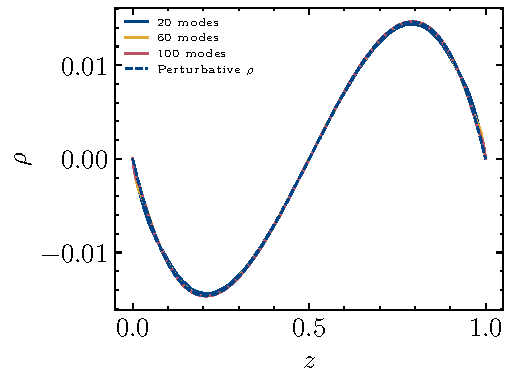
\includegraphics[width=1\textwidth]{Figures/dirichlet/unfilteredRhoaa.pdf}
    \end{subfigure}
    \begin{subfigure}{0.5\textwidth}
        \centering
        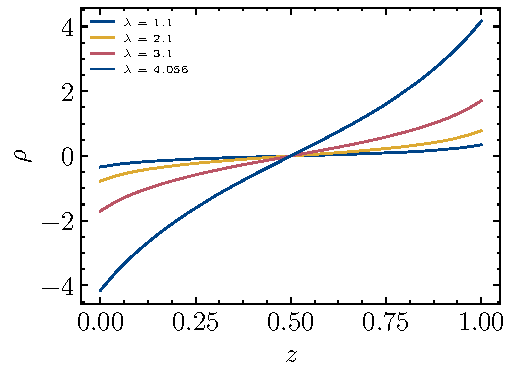
\includegraphics[width=1\textwidth]{Figures/neumann/vacuumPolarizationEvolution.pdf}
    \end{subfigure}
    \caption{The vacuum polarization $\rho$ of the scalar field: In the left
    panel, $m=0$ and using Dirichlet boundary conditions. In the right panel,
    $m=1$ using Neumann boundary conditions.}
    \label{fig:Figures-dirichlet-unfilteredRhoaa-pdf}
\end{figure}

As it was calculated in \cite[]{Wernersson:2020xeh} the vacuum polarization as
defined through point-spliting with respect to $H^{\phi\phi^*}$ yields
\begin{align}
    \rho = \lim_{\tau \to 0} \sum_{n>0}^{} (\omega_n - \varepsilon A_0) \lvert
    \phi_n\rvert^2 e^{-i\omega_n \tau} +\sum_{n<0}^{} (\omega_n - \varepsilon
    A_0) \lvert \phi_n\rvert^2 e^{i\omega_n \tau} + \frac{\varepsilon^2}{\pi}
    A_0 .
    \label{eq:vacuum-polarization-long}
\end{align}
Two examples of $\rho$ calculated using this expression are shown in
Fig.~\ref{fig:Figures-dirichlet-unfilteredRhoaa-pdf}\marginnote{Obviously need
to be redone.}. These are calculated with a constant background electric field
(the external field approximation explained below), with the corresponding mass
and boundary conditions explained in the caption.

To measure the \textit{strength} of the vacuum polarization, the induced charge
\begin{align}
    Q_I = \int_{0}^{\frac{1}{2}} \rho(z) dz
    \label{eq:polarized charge}
\end{align}
is defined. This charge will screen the background electric field $\lambda$,
and Gauß's law yields that the total electric field at $z=\frac{1}{2}$ is
$\lambda + Q_I$.

\subsection{External Field Approximation and critical $\lambda$}
\label{subsec:External-Field-Approximation}

The external field approximation ignores the contribution of the backreaction
of the charged scalar field to the background electric field. This
approximation displays the instabilities of the system, which the inclusion of
backreaction aims to avoid. Thus, Eq.~\eqref{eq:mode-equation} is solved with
$A_0(z) = -\lambda (z - \frac{1}{2})$, and takes the form
\begin{figure}[t]
    \centering
    \begin{subfigure}{0.45\textwidth}
        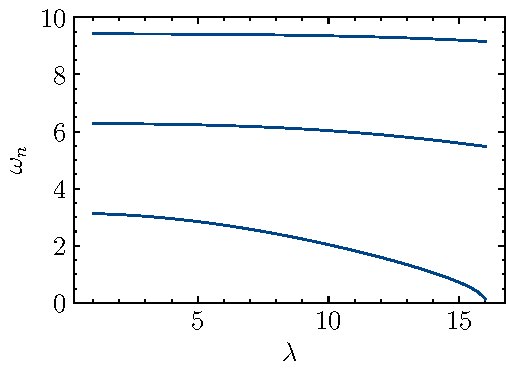
\includegraphics[width=\textwidth]{Figures/dirichlet/eigenvaluesExternalFieldApproximation.pdf}
    \end{subfigure}
    \begin{subfigure}{0.45\textwidth}
        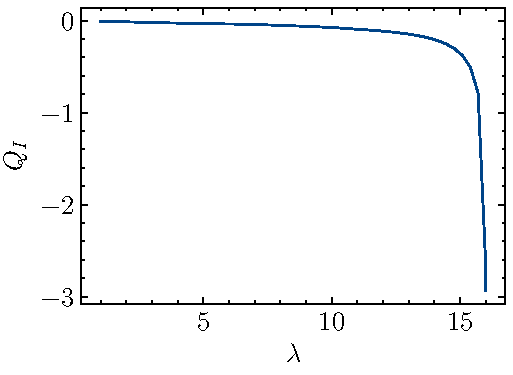
\includegraphics[width=\textwidth]{Figures/dirichlet/inducedChargeExternalFieldApproximation.pdf}
    \end{subfigure}
    \caption{Left panel: Energy of the three first modes of the massless
    Klein-Gordon field with Dirichlet boundary conditions
    corresponding to different values of the dimensionless backgroud
    electric field strength $\lambda.$ Note the apparition
    of $\lambda_c \approx 16.05$ where $\omega_n \to 0.$
Right panel: Corresponding induced charge $Q_I$ as a function of $\lambda$.}
    \label{fig:eigenvalues-external-field-approximation}
\end{figure}
\begin{align}
    \left[ \left(\omega_n + \lambda \left(z-\frac{1}{2}\right) \right)^2 +
    \frac{d {^2}}{d {z^2}} - a^2m^2
\right] \phi_n = 0.  
\label{eq:external-field-approximation-kg}
\end{align}
For each value of $\lambda$, the modes $\phi_n$ and their energies  $\omega_n$ 
can be obtained from the boundary value problem\footnote{The mode solution can 
in fact be written as a linear combination of parabolyc cylinder functions,
as Eq.~\eqref{eq:external-field-approximation-kg} can be rewritten as the Weber equation \cite[]{Ambjorn:1981xv}.}. 
Fig.~\ref{fig:eigenvalues-external-field-approximation} displays the energies
$\omega_n$ of the first three modes $\omega_1, \omega_2, \omega_3$ of the
massless scalar field with Dirichlet boundary conditions as functions of the
background field strength $\lambda$. Notice how the lower curve, corresponding to
$\omega_1$, drops to  $0$ at $\lambda \approx 16$. At that same value of
$\lambda$, the induced charge diverges, as displayed in the left panel of
Fig.~\ref{fig:eigenvalues-external-field-approximation}. This behaviour defines
the critical $\lambda_c$, which adopts different values for different boundary
conditions and masses. As seen in \cite[]{Ambjorn:1981xv}, $\lambda>\lambda_c$
leads to complex mode energies and thus instabilities.

%The modes $\phi_n$ and their
%energies $\omega_n$ can easily be calculated as a boundary
%value problem.	The energies $\omega_n$ of the first three
%modes are displayed for $m=0$ and Dirichlet boundary conditions in
%Fig.~\ref{fig:eigenvalues-external-field-approximation}, as functions of
%the background field strength $\lambda$. The lower curve, corresponding
%to $\omega_1$, drops to  $0$ at $\lambda \approx 16$. This defines
%the critical $\lambda_c$, which appears also for $m\neq 0$ and other
%boundary conditions. As shown by \cite[]{Ambjorn:1981xv}, for values
%$\lambda>\lambda_c$, some frequencies $\omega_n$ turn complex, which
%from the single frequency ansatz leads to runaway solutions.
%
It is claimed in \cite[]{Ambjorn:1981xv}, that the inclusion of
backreaction avoids these instabilities. However, the expression used
for the vacuum polarization is incorrect and one should rather use the
prescription described in \cite[]{Wernersson:2020xeh}. This article
answers the following question: does considering the backreaction
using the correct prescription for the vacuum polarization avoid the
instabilities that would otherwise be present?


%Fig.~\ref{fig:eigenvalues-external-field-approximation} displays the
%energy of the first three modes of the massless Klein-Gordon field with
%Dirichlet boundary conditions\marginnote{Look for a nice abbreviation
%of this. MDBCs? MD KG field?} for different values of $\lambda$ is
%shown. Shows the appearance of $\lambda_c$ as $\omega_n \to 0$, which
%corresponds to $\lambda_c \approx 16$ for this case.


